\documentclass[12pt]{article}

\usepackage{pablo-devoir}
\usepackage{pablo-listings}
\usepackage[a5paper,margin=2cm]{geometry}

\pagestyle{empty}

\title{(In)Équation\\Espace}
\date{5/11/14}
\classe{2\up{des}14}
\dsnum{DS 2}

\begin{document}

\maketitle

\begin{exercice}[Développement et Factorisation --- 6 points]
  On considère la fonction définie par $f(x)=\left( x+1 \right)^2+\left( x+1 \right)\left( x-2 \right)$.

  \begin{enumerate}[(1)]
    \item \begin{enumerate}

        \item Montrer que $f(x)=\left( x+1 \right)\left( 2x-1 \right)$.
        \item Montrer que $f(x)=2x^2+x-1$.
      \end{enumerate}
    \item \begin{enumerate}
        \item Résoudre $f(x)=0$.
        \item Résoudre $f(x)=-1$.
      \end{enumerate}
  \end{enumerate}
\end{exercice}

\begin{exercice}[Inéquations --- 6 points]
  Résoudre (si nécessaire) chacun des couples d'inéquations suivant, et présenter les solutions sur la droite des réels, puis sous forme d'intervalle.
  \begin{enumerate}[(1)]
    \item $2x+1>3+x$
    \item $x<2$ ou $x>3$
    \item $x<3$ et $x>2$
  \end{enumerate}
\end{exercice}

\pagebreak

\begin{exercice}[Volume --- 6 points]~
  \begin{multicols}{2}
    Un fleuriste souhaite connaître le volume d'un vase qu'il utilise. Ce vase a la forme d'un cône tronqué, c'est-à-dire d'un cône auquel on a enlevé la partie inférieure (voir ci-contre).

    Le rayon du cercle supérieur est 10~cm, celui du cercle inférieur est 6~cm, et les hauteurs sont indiquées sur le schéma.

    \columnbreak

    \begin{center}
      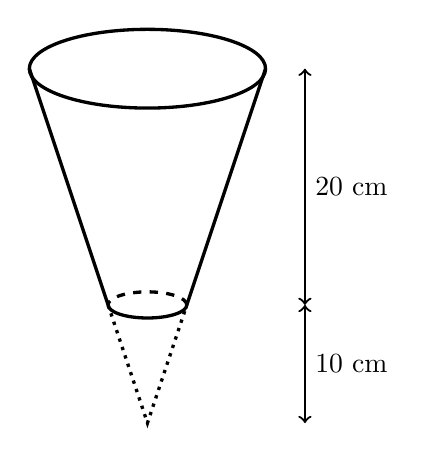
\begin{tikzpicture}[very thick]
        \draw[] (1,0) -- (0,3);
        \draw[] (2,0) -- (3,3);
        \draw[] (1.5,3) ellipse (1.5 and 0.5);
        \draw[dashed] (2,0) arc (0:180:0.5 and 0.166);
        \draw[] (1,0) arc (180:360:0.5 and 0.166);

        \draw[dotted] (1,0) -- (1.5,-1.5) -- (2,0);

        \draw[thick,<->] (3.5,3)
            -- (3.5,0)    node[midway,right]{20~cm};
        \draw[thick,<->] (3.5,0)
            -- (3.5,-1.5) node[midway,right]{10~cm};
      \end{tikzpicture}
    \end{center}
  \end{multicols}

  Les résultats seront arrondis au dixième.
  \begin{enumerate}[(1)]
    \item Calculer le volume du grand cône (avant suppression de la partie tronquée).
    \item Calculer le volume de la partie tronquée (en pointillés sur la figure).
    \item En déduire le volume du vase.
  \end{enumerate}

\end{exercice}

\begin{exercice}[Problème ouvert --- 2 points]\emph{Toute trace de recherche, même incomplète, sera prise en compte dans la notation.}
  \begin{multicols}{2}
    \noindent On considère le cube $ABCDEFGH$, de côté 2~cm. Le point $I$ est le centre de la face $AEFB$ ; $J$ est le centre de la face $CGFB$. Quelle est la longueur du segment $[IJ]$ ?

    \begin{center}
      \begin{tikzpicture}[scale=2,line width=1pt]
        \coordinate (O) at (0,0);
        \coordinate (x) at (1,0);
        \coordinate (y) at ({0.8*cos(30)},{0.8*sin(30)});
        \coordinate (z) at (0,1);

        \coordinate (A) at (O);
        \coordinate (B) at ($(O) + (x)$);
        \coordinate (C) at ($(O) + (x) + (y)$);
        \coordinate (D) at ($(O) + (y)$);
        \coordinate (E) at ($(O) + (z)$);
        \coordinate (F) at ($(O) + (z) + (x)$);
        \coordinate (G) at ($(O) + (z) + (x) + (y)$);
        \coordinate (H) at ($(O) + (z) + (y)$);
        \coordinate (I) at ($(O) + 0.5*(x) + 0.5*(z)$);
        \coordinate (J) at ($(O) + (x) + 0.5*(y) + 0.5*(z)$);

        \draw (A) node[below left]{$A$};
        \draw (B) node[below right]{$B$};
        \draw (C) node[right]{$C$};
        \draw (D) node[below]{$D$};
        \draw (E) node[left]{$E$};
        \draw (F) node[above]{$F$};
        \draw (G) node[right]{$G$};
        \draw (H) node[above]{$H$};
        \draw (A) -- (B) -- (C) -- (G) -- (H) -- (E) -- (F) -- (B);
        \draw (A) -- (E);
        \draw (F) -- (G);
        \draw[dashed] (D) -- (H);
        \draw[dashed] (D) -- (A);
        \draw[dashed] (D) -- (C);

    %\draw[dotted] (A) -- (F) -- (C);
        \draw (I) node{$\times$} node[above left]{$I$};
        \draw (J) node{$\times$} node[above right]{$J$};
        \draw[dotted] (I) -- (J);
      \end{tikzpicture}
    \end{center}
  \end{multicols}
\end{exercice}
\end{document}
